\section{Conclusion and Future Work}
We are the first to evaluate variants of the proportional response algorithm against existing iterative methods for density decomposition. Inspired by momentum-based optimization, we propose \prexp, a novel algorithm with exponential momentum.

\prexp outperforms competitors by orders of magnitude in accuracy across large real-world graphs, demonstrating the effectiveness of exponential momentum. While prior work (Birnbaum et al. ~\cite{DBLP:conf/sigecom/BirnbaumDX11}) suggested linear momentum (\prlin), our results show that \prexp is more promising—though its theoretical analysis remains an open challenge due to its unique combination of gradient descent and exponential momentum.

In summary, \prexp advances density decomposition for large graphs, offering a robust alternative and motivating further research into momentum-based methods.

\ignore{
\begin{acks}

\end{acks}
}


%\begin{figure}[!h] % 强制优先处理
%\begin{figure*}[bp]
\begin{figure}[H]
	\centering
	\begin{subfigure}[b]{\textwidth}
		\centering
		% ???????????
		\begin{minipage}[b]{0.05\textwidth}
			\centering
			\raisebox{1.5cm}{
				\tiny % ????????????
				\renewcommand{\baselinestretch}{0.8}\selectfont % ?????
				\begin{tabular}{c}
					W \\
					E \\
					B \\
					\vrule\\
					G  \\
					O  \\
					O  \\
					G  \\
					L  \\
					E  \\
				\end{tabular}
			}
			%\raisebox{1.5cm}{\rotatebox{90}{\textbf{Main Title}}} % ?????????
		\end{minipage}%
		% ?????
		\begin{minipage}[b]{0.3\textwidth}
			\centering
			\includegraphics[width=\textwidth]{images/parameters/web-google/Absolute_Error_vs_T.png} % ?????????
			
		\end{minipage}%
		% ?????
		\begin{minipage}[b]{0.3\textwidth}
			\centering
			
			\includegraphics[width=\textwidth]{images/parameters/web-google/Multiplicative_Error_vs_T.png} % ?????????
			
		\end{minipage}%
		% ?????
		\begin{minipage}[b]{0.3\textwidth}
			\centering
			
			\includegraphics[width=\textwidth]{images/parameters/web-google/inv_vs_T.png} % ?????????
		\end{minipage}
	\end{subfigure}
	%CATS
	\begin{subfigure}[b]{\textwidth}
		\centering
		% ???????????
		\begin{minipage}[b]{0.05\textwidth}
			\centering
			\raisebox{1.5cm}{
				\tiny % ????????????
				\renewcommand{\baselinestretch}{0.8}\selectfont % ?????
				\begin{tabular}{c}
					W \\
					I \\
					K \\
					I \\
					\vrule\\
					T\\
					O\\
					P\\
					C\\
					A\\
					T\\
					S
				\end{tabular}
			}
			%\raisebox{1.5cm}{\rotatebox{90}{\textbf{Main Title}}} % ?????????
		\end{minipage}%
		% ?????
		\begin{minipage}[b]{0.3\textwidth}
			\centering
			\includegraphics[width=\textwidth]{images/parameters/wiki-cats/Absolute_Error_vs_T.png} % ?????????
			
		\end{minipage}%
		% ?????
		\begin{minipage}[b]{0.3\textwidth}
			\centering
			
			\includegraphics[width=\textwidth]{images/parameters/wiki-cats/Multiplicative_Error_vs_T.png} % ?????????
			
		\end{minipage}%
		% ?????
		\begin{minipage}[b]{0.3\textwidth}
			\centering
			
			\includegraphics[width=\textwidth]{images/parameters/wiki-cats/inv_vs_T.png} % ?????????
		\end{minipage}
	\end{subfigure}
	%%%%%
	\caption{Approximation Quality vs Number of Iterations for \prexp with Different $C$ in 
		$\gamma_t = 1 - \frac{C}{t+C}$, for $C = 1, 2, \ldots, 6$
	}
	\label{fig:parameter_normal_graphs}
\end{figure}



% Articles V3mod140-V3mod259 use
\received{October 2024}
\received[revised]{January 2025}
\received[accepted]{February 2025}


\ignore{
We are the first to evaluate the empirical performance of variants of the well-known proportional response algorithm against existing iterative algorithms based on the quadratic program for the density decomposition. Inspired by first-order methods with momentum, we introduce the novel \prexp algorithm with exponential momentum.

Our findings reveal that \prexp demonstrates the best empirical performance across many large real-world graphs, often outperforming the closest competitor by several orders of magnitude in terms of accuracy. 
%This significant improvement highlights the potential of exponential momentum in enhancing algorithmic efficiency and effectiveness.
Furthermore, our empirical results indicate that momentum methods can enhance the convergence rates of the proportional response algorithm, providing further validation for the idea proposed by Birnbaum et al.~\cite{DBLP:conf/sigecom/BirnbaumDX11}.
However, instead of the conventional linear momentum variant \prlin, a more promising direction for future research would be to perform theoretical analysis on the exponential momentum variant \prexp,
\newtext{which would
	require novel tools as it essentially combines a
	linear gradient descent step with an exponential momentum step. To the best of our knowledge,
	this approach is unprecedented, thereby posing a unique challenge.
}


In conclusion, the introduction of \prexp represents a significant advancement in approximation algorithms for density decomposition in large-scale graphs. It offers a robust alternative to existing methods and paves the way for further exploration and optimization of momentum-based algorithms.
}

